\begin{frame}{Otázky oponenta}
    \begin{block}{Otázka 1a)}
        V práci zavádíte zobrazení intenzit Stokesova vektoru plně polarizovaného světla na
        Poincarého sféře (obr. 1.3).
        V práci dále řešíte odezvu optického můstku sestávajícího z fázové destičky, polarizačního děliče a dvojice detektorů, přičemž můstek je nastaven tak, aby rozdíl signálů z obou detektorů byl nula (kapitola 4.2).
        Množina polarizací, které poskutují nulový signál z ideálního optického můstku je pak znázorněna poledníkem mezi pólem kruhových polarizací a polarizací 0-\SI{90}{\degree} (obr. 4.3).
        Můžete prosím graficky ukázat, jak se tato množina nulové odezvy změní, když můstek nebude sestaven z opticky ideálních elementů?
        Např. když zpoždění fázové destičky nebude přesně $\pi/2$, či fázová destička bude mít různou propustnost pro obě vlastní polarizace?
    \end{block}
\end{frame}

\begin{frame}{Otázky oponenta}
    \begin{block}{Otázka 1a)}
        [Množiny nulové odezvy pro neideální fázovou destičku?]
    \end{block}
    \begin{exampleblock}{Odpověď 1a)}
        \begin{columns}
            \begin{column}{0.5\textwidth}
                \begin{itemize}
                    \item Nepřesné fázové zpoždění
                    \item Vyklopení do $s_3$ 
                \end{itemize} 
                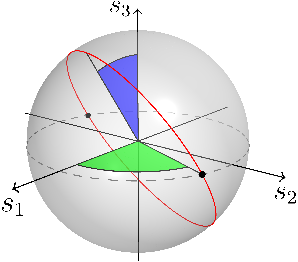
\includegraphics[width=4cm]{img/kovek-4.pdf}
            \end{column}
            \begin{column}{0.5\textwidth}
                \begin{itemize}
                    \item Rozdílná propustnost
                    \item Posunutí v rovině $s_1s_2$
                \end{itemize} 
                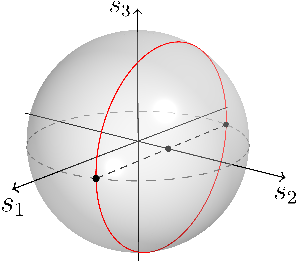
\includegraphics[width=4cm]{img/kovek-6.pdf}
            \end{column}
        \end{columns}
    \end{exampleblock}
\end{frame}

\begin{frame}{Otázky oponenta}
    \begin{block}{Otázka 1b)}
        Jak se v této vizualizaci projeví, když např. k s-polarizovanému světlu na vstupu (($\beta=0$) a optický můstek je vyvážen) je přičtena např. Kerrova rotace a optický můstek tedy přestane být vyvážen?
    \end{block}
    \begin{exampleblock}{Odpověď 1b)}
        \begin{itemize}
            \item Stokesův kovektor zůstane nezměněný -- stav detekční aparatury (můstku) se nezměnil
            \item Změní se Stokesův vektor -- vstupní světlo se změnilo právě o Kerrovu rotaci
            \item Detekovaný signál je dán ``vzdáleností'' bodu od kružnice
        \end{itemize}
    \end{exampleblock}
\end{frame}

\begin{frame}{Otázky oponenta}
    \begin{block}{Otázka 1b)}
        [Jak se projeví Kerrova rotace (rozvážení můstku)?]
    \end{block}
    
    \begin{exampleblock}{Odpověď 1b)}
        \begin{columns}
            \begin{column}{0.5\textwidth}
                \begin{itemize}
                    \item Nepřesné fázové zpoždění
                    \item Vyklopení do $s_3$ 
                    \item V signálu se projeví elipticita
                \end{itemize} 
                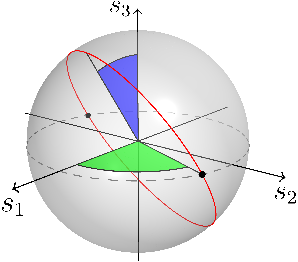
\includegraphics[width=4cm]{img/kovek-4.pdf}
            \end{column}
            \begin{column}{0.5\textwidth}
                \begin{itemize}
                    \item Rozdílná propustnost
                    \item Posunutí v rovině $s_1s_2$
                    \item Snížení faktoru stočení
                \end{itemize} 
                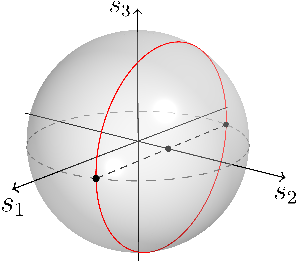
\includegraphics[width=4cm]{img/kovek-6.pdf}
            \end{column}
        \end{columns}
    \end{exampleblock}
\end{frame}

\begin{frame}{Otázky oponenta}
    \begin{block}{Otázka 2)}
        Při zpracování magnetooptických spekter CoFe je oddělena magnetooptická odezva (např. určení spekter amplitudy a anizotropie magnetooptického jevu) a magnetická odezva (určení snadných os a magnetické anizotropie), obr. 5.2.
        V tomto zpracování je magnetická anisotropie určena pro různé vlnové délky světla, což není fyzikálně přesné, ale indikuje správnost oddělení obou jevů.
        Bylo by možné modifikovat formalismus zpracování dat, aby bylo zcela odděleno magnetické chování vzorku (tj. stejné chování pro všechny vlnové délky světla) a magneto-optická spektrální odpověď vzorku?
    \end{block}
\end{frame}
\begin{frame}{Otázky oponenta}
    \begin{block}{Otázka 2)}
        [Oddělené zpracování magnetické a magneto-optické odezvy?]
    \end{block}
    
    \begin{exampleblock}{Odpověď 2)}
        \begin{itemize}
        \item Analýza $\equiv$ globální minimalizace chybové funkce $\mathcal{L} = \sum \left( U_{\textrm{experiment}} - U_{\textrm{model}} \right)^2$, kde $U_{\textrm{model}}(\textrm{M},\,\textrm{MO})$
        \item Je možné zpracovávat všechny vlnové délky zároveň, pak $U_{\textrm{model}}(\textrm{M},\,\textrm{MO}(\lambda_1),\,\textrm{MO}(\lambda_2),\,\ldots)$
                \begin{itemize}
                    \item Různé $\lambda$ mají různou hladinou šumu, je nutné to zohlednit přidáním vah do chybové funkce $\mathcal{L}=\sum_\lambda w^2(\lambda) \left(U_{\textrm{experiment}} - U_{\textrm{model}}\right)^2$
                    \item Pokud jsou výsledky podobné (v jejich rozsahu je model přibližně lineární) je to ekvivalentní váženému průměru výsledků jednotlivých $\lambda$
                    \item Vyzkoušeno, ale kvůli předchozímu bodu nepoužíváno
                \end{itemize}
        \end{itemize}
    \end{exampleblock}
    
\end{frame}


